\newcommand{\ass}{Robotic systems\\ Report}
\newcommand{\name}{Sergio Castillo\\ Vince Jankovics\\ Mike Lagunes\\ Kevin Zhou}

\documentclass[12pt,a4paper]{article}
\usepackage[utf8]{inputenc}
\usepackage[english]{babel}
\usepackage{amsmath}
\usepackage{amssymb}
\usepackage{amsthm}
%\usepackage{graphicx}
\usepackage[usenames,dvipsnames]{xcolor}
\usepackage{color}
%\usepackage{graphicx}

%\usepackage{natbib}
%\bibliographystyle{agsm}
%\usepackage[backend=bibtex,style=authoryear,sorting=nyt,maxcitenames=2,uniquelist=false]{biblatex}
\usepackage[backend=bibtex]{biblatex}
\addbibresource{ref.bib} % note the .bib is required


\usepackage{listings}
\lstset{language=matlab,tabsize=3,backgroundcolor=\color{light-gray}}
\lstset{commentstyle=\color{Sepia},numbers=left,stepnumber=5}
\lstset{keywordstyle=\color{MidnightBlue}\bfseries\emph,
stringstyle=\color{Mulberry},
numberstyle=\color{gray},
tabsize=2,
caption=\lstname,
breaklines=true,
identifierstyle=\color{Mahogany}}

\usepackage{enumitem}
\setlist{noitemsep} % or \setlist{noitemsep} to leave space around whole list


%\usepackage{cite}
\usepackage{hyperref}
\hypersetup{
 colorlinks,
 citecolor=Black,
 linkcolor=Black,
 urlcolor=Blue}
 
\usepackage{ifpdf}
\ifpdf
\usepackage[pdftex]{graphicx}
\graphicspath{{./fig/}}
\usepackage[outdir=./]{epstopdf}
\epstopdfDeclareGraphicsRule{.eps}{pdf}{.pdf}{%
ps2pdf -dAutoRotatePages/None -dEPSCrop #1 \OutputFile
}
\else
\usepackage{graphicx}
\fi
%\epstopdfDeclareGraphicsRule{.gif}{png}{.png}{convert gif:#1 png:\OutputFile}
%\AppendGraphicsExtensions{.gif}

\usepackage{pst-all} 



%\usepackage{tikz}
\usepackage{caption}
\usepackage{subcaption}
\usepackage{placeins}
%\usepackage{subfig}
\usepackage{float}

\usepackage{fullpage}


\newcommand{\tab}{\hspace*{15pt}}

\definecolor{light-gray}{gray}{0.95}

\usepackage{fancyhdr}
\setlength{\headheight}{0pt}
\pagestyle{fancy}

%\renewcommand{\theenumi}{\alph{enumi}}

\newcommand{\vc}[1]{\mathbf{#1}}

%\renewcommand{\sectionmark}[1]{}
%\renewcommand{\chaptermark}[1]{}
%\renewcommand{\refname}{}
\renewcommand{\subsectionmark}[1]{}  
\renewcommand{\headrulewidth}{0pt}
\fancyhead{}
\rhead{}
\rfoot{}
\lhead{}

%\usetikzlibrary{calc}

\newcommand*{\titleM}{
\thispagestyle{empty}
\newlength{\drop}
\begingroup% Misericords, T&H p 153

%\begin{tikzpicture}[remember picture, overlay]
%    \node[inner sep=0pt] at (current page.center){%
%        \includegraphics[width=\paperwidth]{header6.png}%
%    };%
%\end{tikzpicture}

\drop = 0.18\textheight
\centering
\vspace*{\drop}
\vspace*{\drop}
{\Huge\bfseries \ass}\\[\baselineskip]
{\large\scshape \name}\par
\vfill
\vspace*{2\drop}
%\pagebreak
\endgroup

\thispagestyle{empty}
\makebox[\textwidth]{}
\pagebreak
\makebox[\textwidth]{}
\setcounter{page}{1}
}

\newcommand{\figs}{0.9}
\newcommand{\dt}{\mathrm{d}t}
\newcommand{\der}[1]{\frac{\mathrm{d}#1}{\dt}}
\newcommand{\F}[1]{\mbox{Figure \ref{#1}}}
\newcommand{\comment}[1]{\textit{\textcolor{Green}{#1}}}
\newcommand{\question}[1]{\textit{\textcolor{Red}{#1}}}
\headsep = 25pt

\renewcommand{\qedsymbol}{$\blacksquare$}
%\setlength\itemsep{0em}
%\renewcommand{\thesubsection}{\Alph{subsection})}
\renewcommand{\c}[1]{\mathrm{c}\left(#1\right)}
\newcommand{\s}[1]{\mathrm{s}\left(#1\right)}
\newcommand{\atan}[1]{\mathrm{atan2}(#1)}
\newcommand\SmallMatrix[1]{{%
%  \footnotesize
  \scriptsize \arraycolsep=0.8\arraycolsep\ensuremath{\begin{bmatrix}#1\end{bmatrix}}}}

\begin{document}
	\titleM
	
	\section{Introduction}
		
	\documentclass[12pt]{article}
\usepackage{enumitem}
\begin{document}
\section{Robot Design}

During the first stage of the design one beta version using caterpillar wheels and the sensor on the top to turn 360° was created finding some disadvantages that were solved in the last version.

The current version of the robot was developed based on the findings found on the first version and contains the next advantages:

Compact design.

Tail to turn.

Sensor in the front.

\end{document}
	
	\section{Mathematical modelling}
	
		\subsection{Sensors}
		
		\subsection{Actuators}
		
		\subsection{Overall system}
		
		\subsection{Experiments, validation}
		
	\section{The kidnapped robot problem}
	
		\subsection{Localization}
		
		\subsection{Guidance}

	Before and after the robot is localized in the map, it has to know what to do next according to the current objective, which are:
	\begin{enumerate}
		\item Avoid collision all time,
		\item Explore map,
		\item Go to target.
	\end{enumerate}
	
	\subsubsection{Collision avoidence}
	
		The robot's highest priority objective is avoiding collisions with the walls. This is done by a simple algorithm, which estimates the smallest distance between the robot and the scanned points based on the commanded movement. If this predicted distance is smaller than a certain threshold, it 'bounces back' from the boundary (see Figure \ref{fig:ca}). The reflected angle is perturbed with a small noise factor, so the robot does not get stuck in an area (e.g. when it goes perpendicular to the wall).
		
		\begin{figure}[h]
		   \centering
			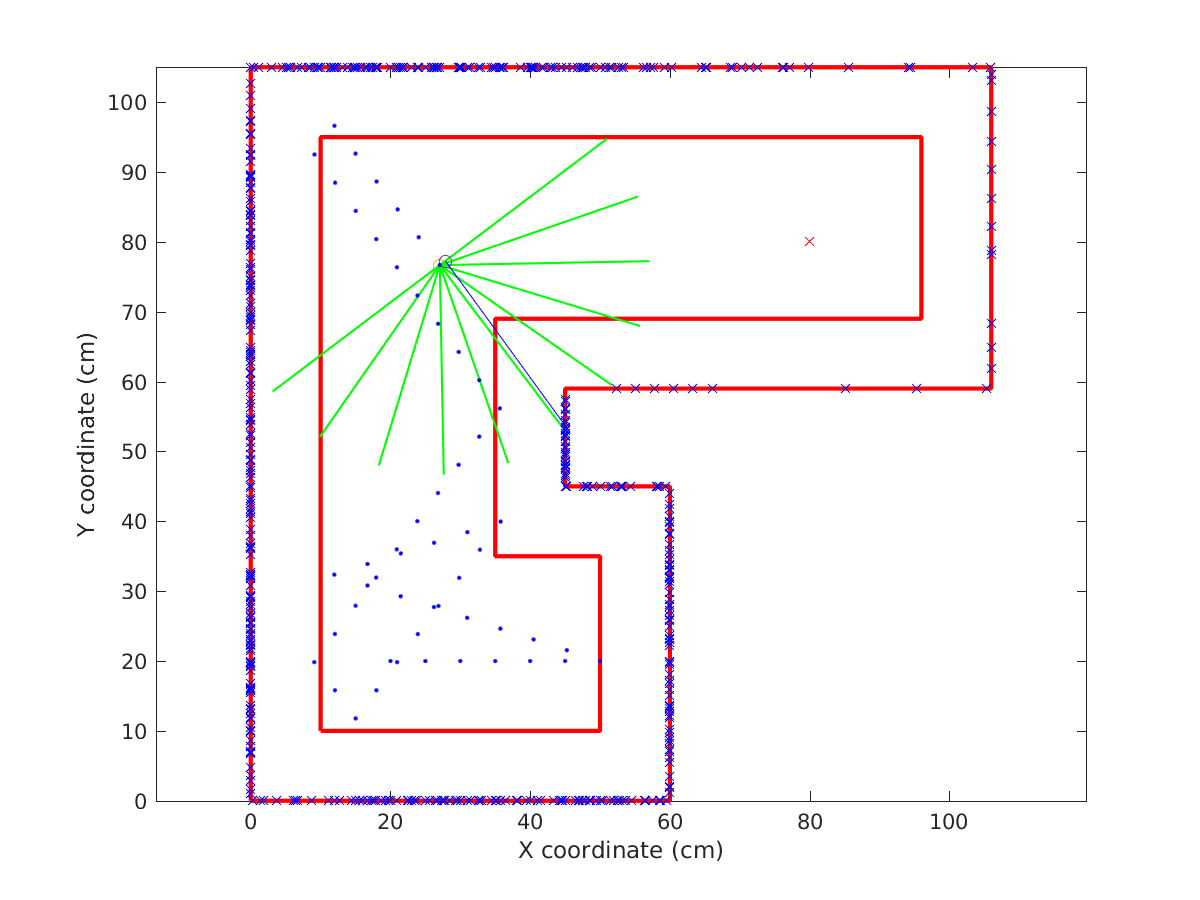
\includegraphics[width=.75\textwidth]{ca1}
		    
		   \caption{'Wall bouncing', with a distance threshold of 10cm (inner boundary).}
		   \label{fig:ca}
	 	\end{figure}
	
	\subsubsection{Exploration}
	
		The exploration is done before the PFL is converged to a location (i.e. the localization is not complete), so the robot can wonder around the map and exploit more of its features. The robot builds an internal map of the sensed points (called {\tt knownPoints} in the code) and the points where it had been (called {\tt beenThere} in the code), which serve as the basis of the decision making. These are based on the commanded movements and sensor data, so they are a rough estimate of the surrounding space. 
		
		The points are used to build an \textit{Artificial potencial field} ($U$), and drive the robot downhill (i.e. $-\nabla U$) \parencite{choset_principles_2005}. Since the points where the robot had been is also used for this field (with different weight than the walls), the robot is driven towards unexplored locations. The result can be seen on Figure \ref{fig:apf}.
		
		\begin{figure}[h]
		    \centering
		    \begin{subfigure}[b]{0.48\textwidth}
   	 			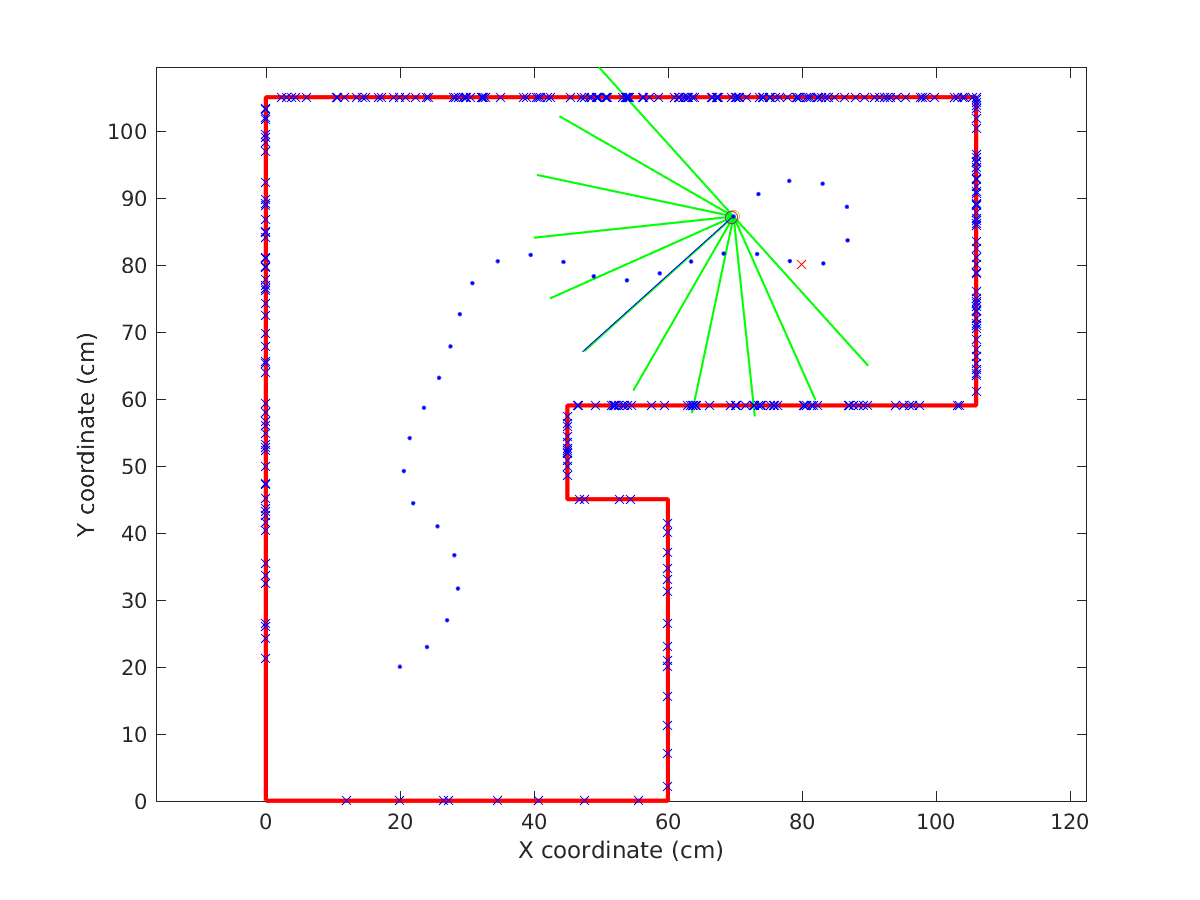
\includegraphics[width=\textwidth]{apf1}
   	 			\caption{}
				\label{fig:apf1}
   	 		\end{subfigure}		    
		    ~
		    \begin{subfigure}[b]{0.48\textwidth}
   	 			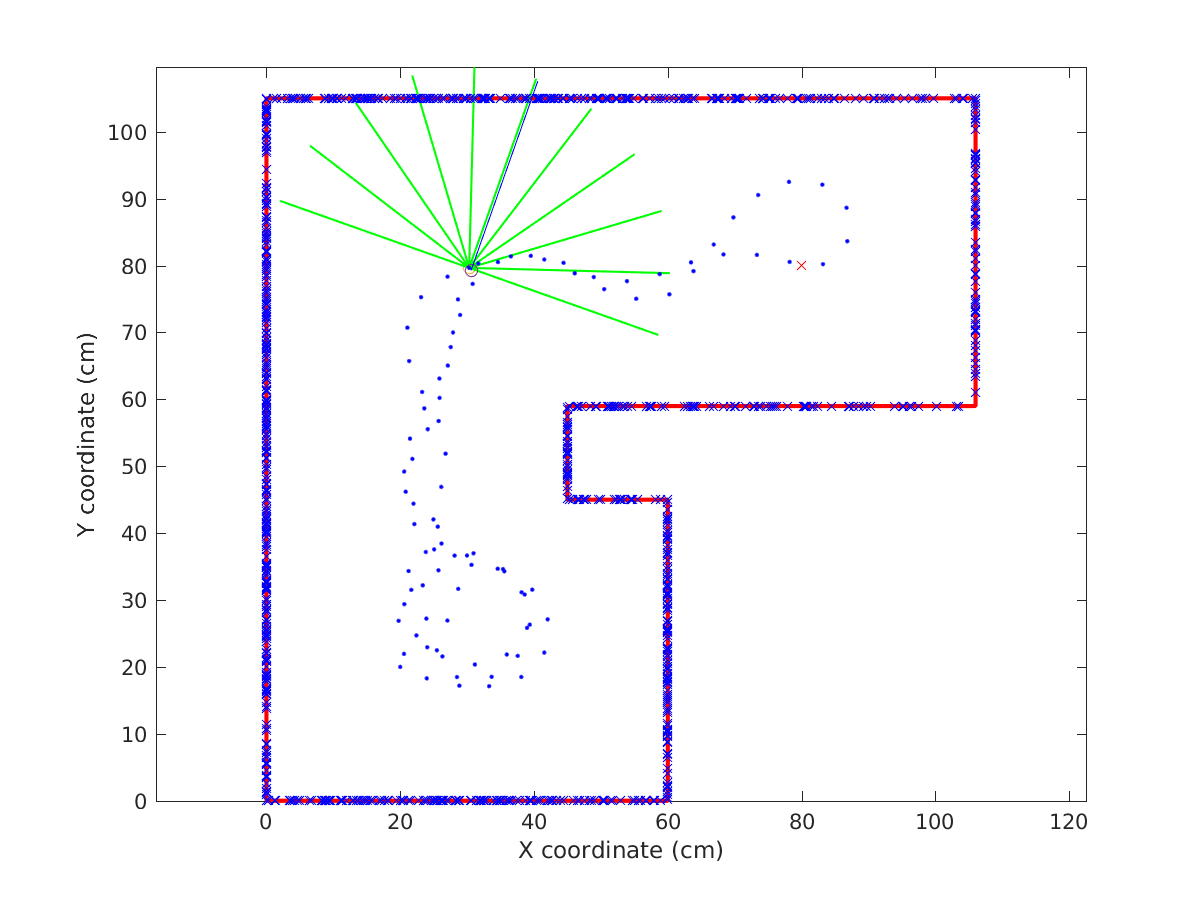
\includegraphics[width=\textwidth]{apf2}
   	 			\caption{}
 				\label{fig:apf2}
   	 		\end{subfigure}
   	 		%		    \subfloat[][]{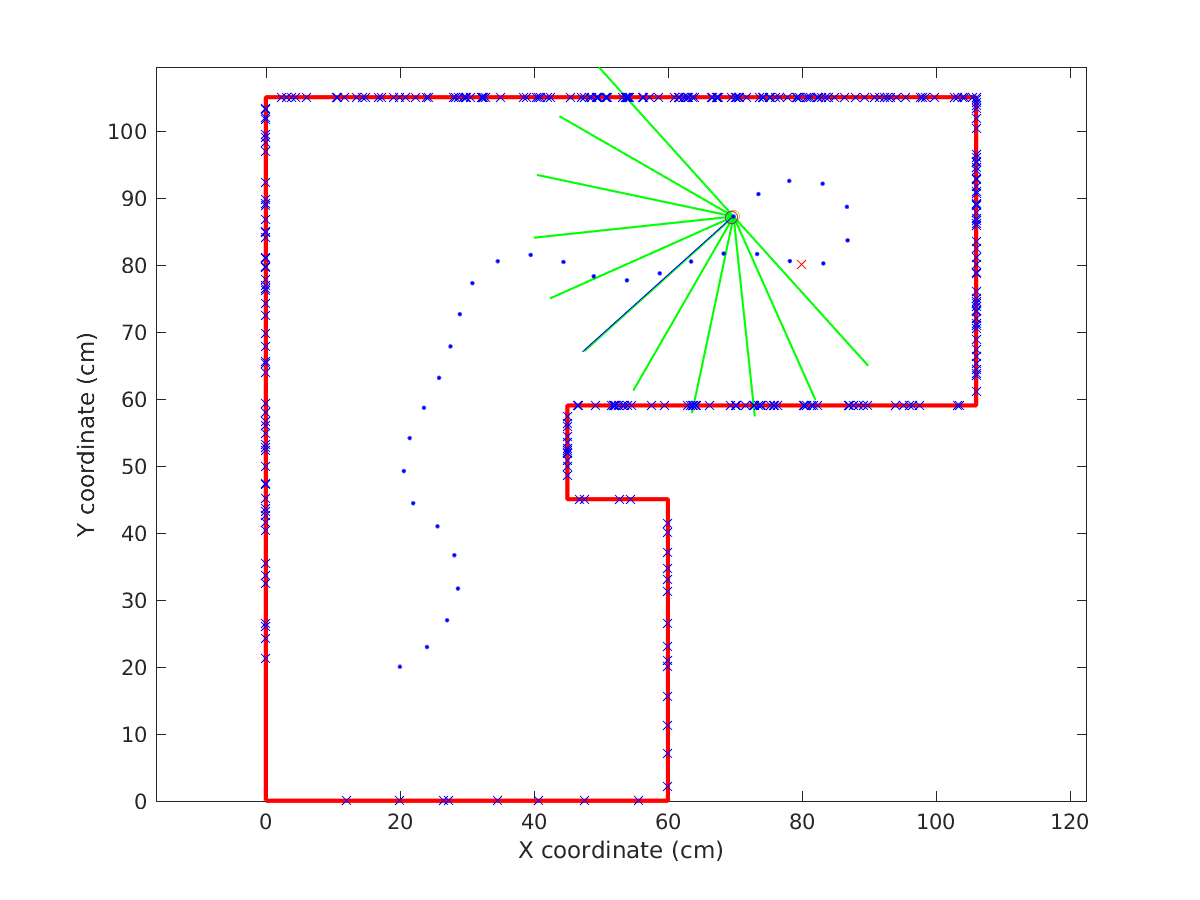
\includegraphics[width=.5\textwidth]{apf1}\label{fig:apf1}}
%		    \subfloat[][]{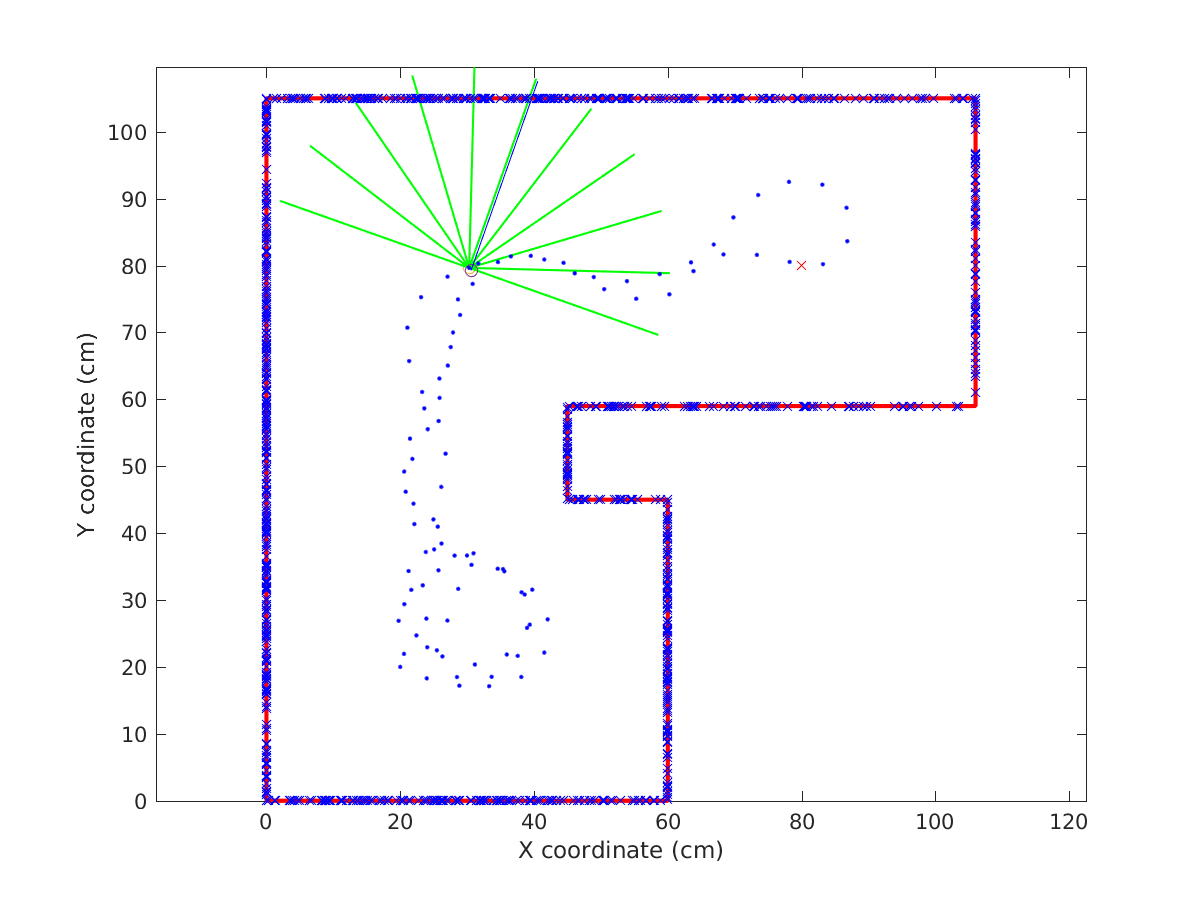
\includegraphics[width=.5\textwidth]{apf2}\label{fig:apf2}}
		     
		    \caption{Simulation with artificial potential field as guidance ($\epsilon=0.3$). (\protect\subref{fig:apf1}) Initial path. (\protect\subref{fig:apf2}) Path after some time.}
		    \label{fig:apf}
	 	\end{figure}
	 	
	 	
	 	
	 	The effect of the potencial field can be tuned by the constant $\epsilon$, so the commanded turning angle is:
	 	\begin{equation}
			\delta \theta=\epsilon\cdot\arg(-\nabla U),
	 	\end{equation}
	 	meaning that with lower $\epsilon$ the robot has higher inertia (goes more uphill). The commanded forward movement is kept constant, so the robot gives more consistent response even on higher gradient values (e.g. close to a wall).
	 	
	 	
	 	This feature improves the robot's movement compared to the simple bouncing, but it needs the collision avoidance as a simple backup. The result is shown on Figure \ref{fig:apf3}.

		
		\begin{figure}[h]
			\centering
			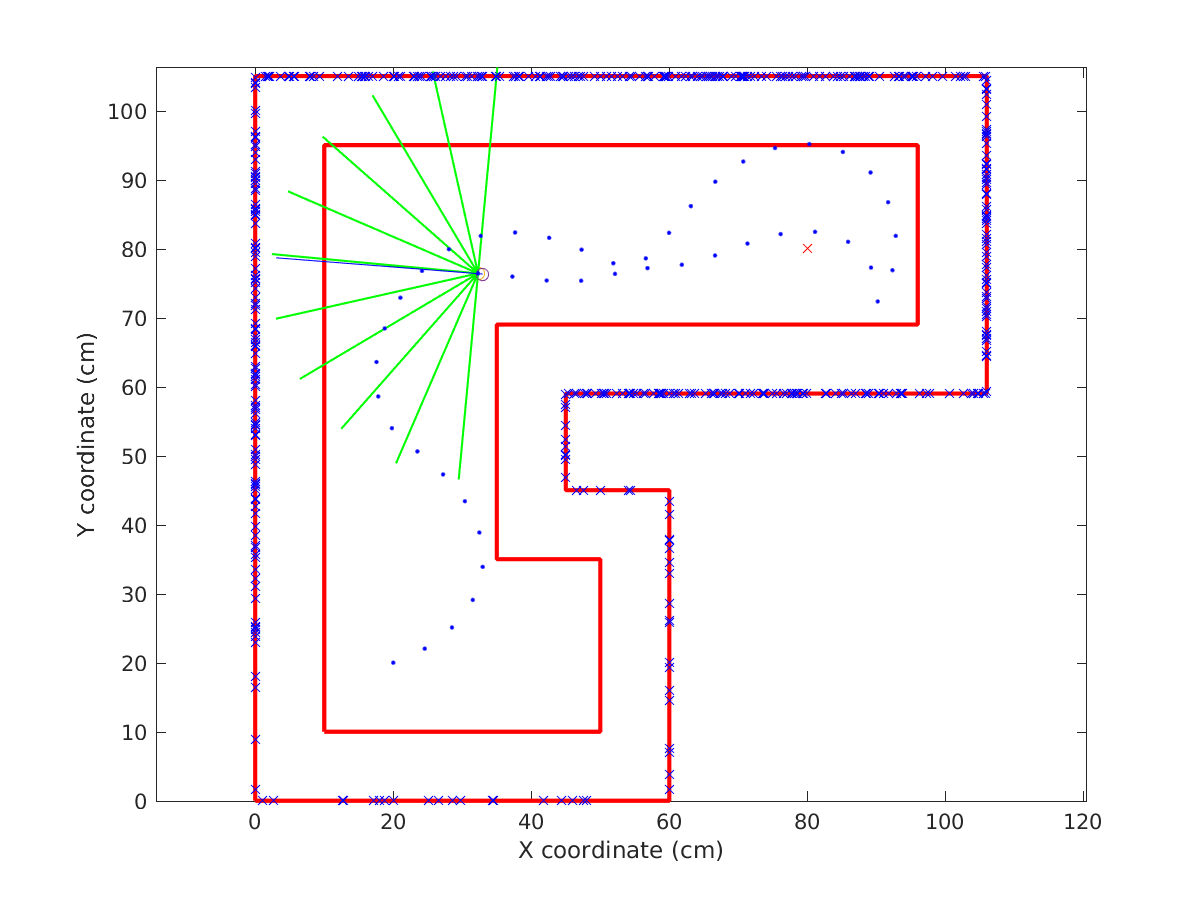
\includegraphics[width=.75\textwidth]{apf3}
			
			\caption{Combined exploration (artificial potential field with $\epsilon=0.2$ and collision avoidance), the former explores the space, a latter makes sure that the robot does not collide with the wall in any circumstances.}
			\label{fig:apf3}
	 	\end{figure}
	 	
	\subsubsection{Path planning} 	
	
		After the PFL is converged, the robot can plan its path from its current location to the target. The planning algorithm was a standard A* search \parencite{introduction_astar} on a visibility graph \parencite{choset_principles_2005} defined by the map, robot and target. This way the search space for the optimal path is greatly reduced and the movements are smoother compared to a grid-word representation. Figure \ref{fig:vm1} shows the visibility graph with the optimal path between the robot and the target.
		
		\begin{figure}[h]
		    \centering
  	 		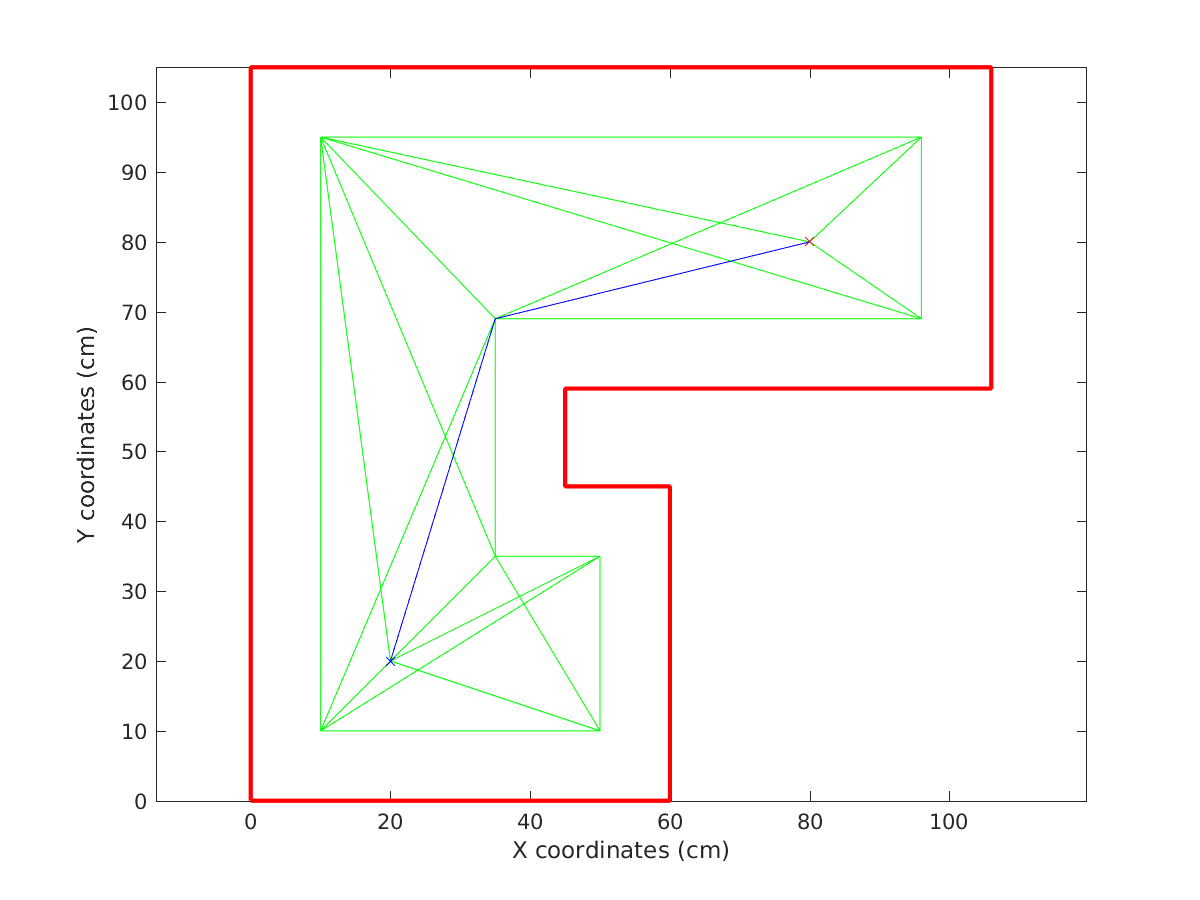
\includegraphics[width=.75\textwidth]{vm1}
		    \caption{A* search on the visibility graph finds the shortest path (blue line) between the robot and the target (blue and red cross respectively). The modified map is used, so the robot does not go closer to the walls than 10cm.}
		    \label{fig:vm1}
	 	\end{figure}
	 	
		\FloatBarrier
 	
 	\section{Results}
 	
 		\subsection{Simulation}
 		
 		\subsection{Experiments}
 		
 	\section{Discussion}
 
 
 
 \printbibliography
 
 \section*{Appendix}
 
 		 	
	 	
\end{document}

